\chapter{Instructions for annotators}

The following document in Czech is what was send (with minor styling edits) to the annotators from the experiment described in \cref{chp:experiment}. It briefly introduces the user interface and the annotation task with an example.

\section*{Ptakopět Pilot Experiment}

Ptakopět je nástroj pro práci s překladačem. Hlavní je levé horní textové pole, obsahující zdrojový text, pravé horní zobrazující text přeložený strojovým překladem a levé spodní, zobrazující zpětný překlad (z cizího jazyka zpět do zdrojového). První dvě zmíněná pole je možné editovat.

\begin{figure}[H]
  \centering
  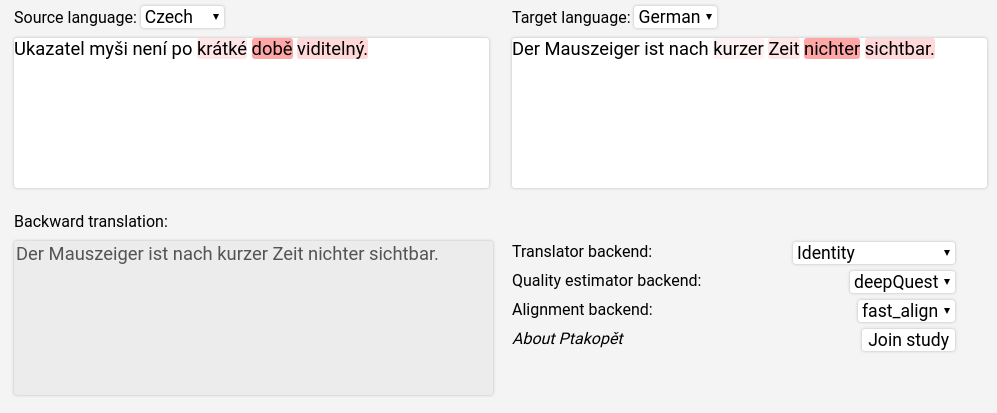
\includegraphics[width=\textwidth]{img/instructions/layout.png}
\end{figure}

Červené zabarvení v druhém poli indikuje, že překlad je v tomto místě nějakým způsobem problematický, jde ovšem o automatický odhad, který může být zavádějící. V prvním okně se pak podbarveně zobrazují slova, která pravděpodobně odpovídají těm problematickým v překladu.

\section*{Studie}

\subsection*{Úvod}

Systém je nasazen na webové adrese: \href{https://ptakopet.vilda.net/}{ptakopet.vilda.net}. Doporučujeme krátké seznámení se systémem mimo samotnou studii. V případě nejasností se, prosím, obraťte na mail \href{mailto:zouhar@ufal.mff.cuni.cz}{zouhar@ufal.mff.cuni.cz}. Studie se týká použití Ptakopětu k překladu do němčiny pro uživatele, kteří německy neumí.

Po celou dobu práce je zapotřebí být připojen k internetu. Po zmáčknutí tlačítka Join study se zobrazí dialog, do kterého je potřeba vložit vaše ID, které jste od nás dostali mailem. Pokud se vám po potvrzení zobrazí hláška Unknown user ID., bylo zadáno špatné ID a je třeba stránku načíst a zadat ID znovu.

\pagebreak

\subsection*{Příklady}

V případě úspěšného přihlášení se zobrazí první z vašich příkladů spolu s krátkou instrukcí. Ty jsou čtyř charakterů:

\begin{enumerate}
    \item Popis daného problému technické podpoře, která komunikuje pouze německy.
    \item Formulace otázky v němčině, na kterou v kontextu věty odpovídá zvýrazněná část českého odborného textu.
    \item Formulace otázky v němčině, na kterou v kontextu věty odpovídá zvýrazněná část anglického odborného textu.
    \item Formulace otázky v němčině, na kterou v kontextu věty odpovídá zvýrazněná část českého administrativního textu.
\end{enumerate}

První druh příkladu obsahuje navíc červené podbarvení, které signalizuje kvalitu překladu, ovšem ne směrodatně. Ukázka příkladu druhého druhu:

\begin{figure}[H]
  \centering
  
\includegraphics[width=\textwidth]{img/instructions/stimuli.png}
\end{figure}

Prvním řešením (pište do prvního textového pole) může být např. \textit{Co bylo rozpuštěno po indickém povstání v roce 1857?} Po překladu se však může ukázat, že různé obraty jsou zpětně špatně přeloženy. V takovém případě je třeba původní otázku nadále reformulovat, dokud nebudete s překladem do němčiny spokojeni (jde samozřejmě jen o váš odhad, německy neumíte).

\subsection*{Pohyb mezi příklady}

Po dokončení práce s konkrétním příkladem klikněte na tlačítko \textit{OK} a zobrazí se další. V případě, že jsou s nějakým příkladem problémy, můžete ji přeskočit tlačítkem \textit{SKIP} v takovém případě je však třeba vhodné udat důvod. Přesnější popisy jsou pro studii přínosnější.

\subsection*{Přerušení}
Váš postup je uchováván v rámci jednoho prohlížeče na jednom zařízení. Tj. zařízení i konkrétní prohlížeč lze vypínat. Po znovunačtení stránky v prohlížeči a zadání uživatelského ID by se měl zobrazit příklad, u které jste naposledy skončili. Informace o aktuálním příkladu bude ztracena v případě smazání historie, cookies, nebo dat z webu (většinou v nastavení prohlížeče).

\subsection*{Konec}

Množství otázek přesahuje váš čas pro tento projekt (zhruba 6 hodin). Až to nastane, napište mail na \href{mailto:zouhar@ufal.mff.cuni.cz}{zouhar@ufal.mff.cuni.cz}. Zde můžete buď skončit, nebo dále pokračovat, dokud nedojde zásoba otázek. Mzda je hodinová a přesný čas, který jste prací s příklady strávili se měří automaticky a ukládá na serveru.

\subsection*{Poznámka}
Během průběhu experimentu jsme stihli zaznamenat jeden technický problém. Některým uživatelům se po 5-10 minutách používání Ptakopětu snižuje responzibilita stránky Ptakopětu. Pokud se vám to stane, načtěte prosím stránku znovu.
Jedná se o technický nedostatek, který se nám bohužel na poslední chvíli nepodařilo odstranit.